\documentclass[11pt, oneside]{article}   	% use "amsart" instead of "article" for AMSLaTeX format
\usepackage{geometry}                		% See geometry.pdf to learn the layout options. There are lots.
\geometry{letterpaper}                   		% ... or a4paper or a5paper or ... 
%\geometry{landscape}                		% Activate for for rotated page geometry
%\usepackage[parfill]{parskip}    		% Activate to begin paragraphs with an empty line rather than an indent
\usepackage{graphicx}				% Use pdf, png, jpg, or eps§ with pdflatex; use eps in DVI mode
								% TeX will automatically convert eps --> pdf in pdflatex		
\usepackage{amssymb}
\usepackage{amsmath}
\usepackage{parskip}
\usepackage{color}
\usepackage{hyperref}

\title{Elementary Theory of Calculus}
%\author{The Author}
%\section{}
%\subsection*{}
\date{}							% Activate to display a given date or no date

\graphicspath{{/Users/telliott_admin/Dropbox/Tex/png/}}
% \begin{center} 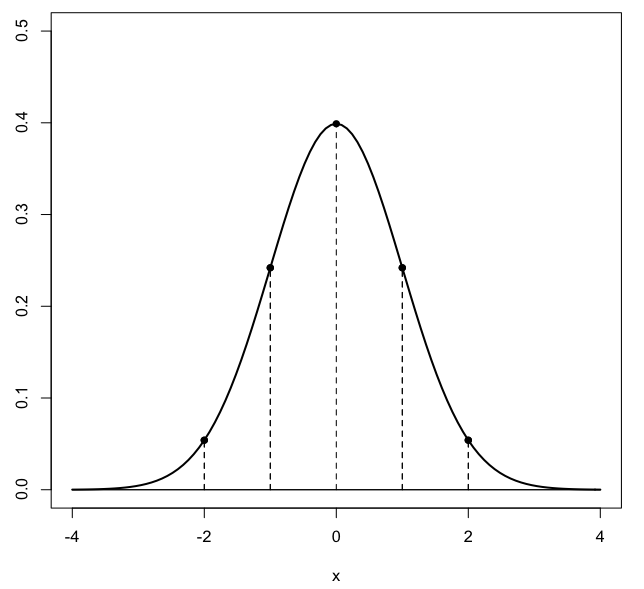
\includegraphics [scale=0.4] {gauss3.png} \end{center}
\begin{document}
\maketitle
\Large
A simple approach to calculus, one suitable for engineers and perhaps even physicists, consists simply of using standard rules like the chain rule and the product rule to calculate derivatives.  We keep track of the derivatives obtained so that when the time comes we can reverse the process to integrate.  In this way a wide variety of interesting and practical problems can be solved.

As Sylvanus Thompson
\begin{center} 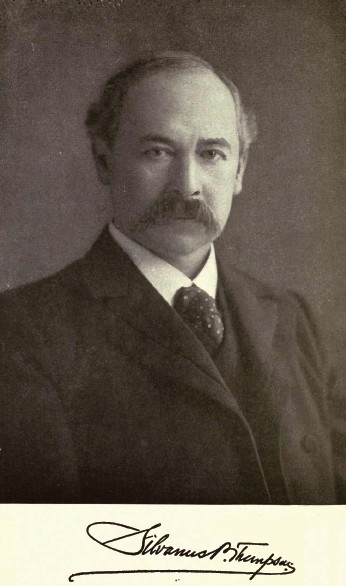
\includegraphics [scale=0.4] {Thompson_Silvanus_mature} \end{center}
 says in his famous book \emph{Calculus Made Easy}, we
\begin{quote}think of $dx$ as a little bit of $x$, and $dt$ as a little bit of $t$\end{quote}
and work with the ratio $dx/dt$ as these quantities become very small.  

We do not require that $dt$ (or $dx$) ever become zero.

We insist only that they become so small that a further reduction in size does not alter the numerical answers we obtain, which are in any case approximations for all physical problems.

Calculus was used with great success in this way by physicists, engineers and even mathematicians for more than a hundred years, and this general approach was still taught to most students until early in the 20th century.

A new method then entered, developed by people such as Cauchy, Bolzano and Weierstrass.  This is a more sophisticated approach, one in which \emph{limits} are emphasized, becoming ever more complicated as the discussion becomes more rigorous.  This is epitomized by the "delta-epsilon game" game we will see later on.  

In addition to rigor, mathematicians also want to know what to do with functions that are not as well-behaved as $f(x) = x^2$.  Some of these are termed "pathological" functions.  An example is
\[ f(x) = 
\begin{cases}
1, \ \ \ x \in \mathbb{Q}, \text{ the set of rational numbers } p/q \\
0, \ \ \ x \notin  \mathbb{Q}, \text{  the irrational numbers}
\end{cases}
\]

You can imagine that the graph of this function looks like a linear hairbrush, with spikes at each rational number, and no spike at the much more numerous irrational numbers.

However, although they are of theoretical interest, such examples don't mean as much to engineers.

\section*{Rational numbers}
Let's start by looking at the properties of numbers, which are subtle and also a bit strange.  This is responsible for much of the complication with calculus.

The set $\mathbb{N}$ are the \emph{natural} or counting numbers $1,2,3 \dots$  The set $\mathbb{Z}$ contains $\mathbb{N}$ plus their negatives, plus $0$.  
\[ \mathbb{Z} = \{ \dots -2, -1, 0, 1, 2, \dots \} \]
$\mathbb{Z}$ stands for the German word \emph{Zahlen}, Numbers.  The set $\mathbb{Z}$ are usually referred to as the integers.

The set $\mathbb{Q}$ (for quotient) are the rational numbers, named not for their reasonableness, instead the name is derived from ratio. 
\[ \mathbb{Q} = \{ \frac{p}{q} \} \text{ for } p \in \mathbb{Z}, q \in \mathbb{N} \]
(Notice that we define $q > 0$).

Finally, the real numbers are represented by the symbol $\mathbb{R}$.

Every rational number can be represented as a decimal, using the method known as long division.

Consider $1/2$
\[ 2 \overline{)1.000} \]
$2$ goes into $10$ exactly $5$ times, generating $0$ remainder and the decimal terminates as $0.5$.

Alternatively, there might be a remainder.

Consider $1/8$.
\[ 8 \overline{)1.000} \]
$\circ$  $8$ goes into $10$ once, leaving $2$ as remainder

$\circ$  $8$ goes into $20$ twice, leaving $4$.  

$\circ$  $8$ goes into $40$ exactly $5$ times with no remainder.

The result is $0.125$.

The other possibility is that in going through the process a remainder comes up that has been seen previously.  If we don't terminate with zero, then this must eventually happen, because there are only as many as $q$ possible remainders.

Thus, for example
\[ 1/7 = 0.142857142857 \dots \]

Conversely, every repeating decimal can be represented as a rational number.  For example

\[ r = 0.142857142857 \dots \]
\[ 1000000 \times r = 142857.142857 \dots \]
\[ 999999 \times r = 142857 \]
\[ r = \frac{142857}{999999} = \frac{1}{7} \]
(since $142857$ goes into $999999$ exactly $7$ times).  You can do this trick with 
\[ r = 0.333 \dots \]
\[ 10 \times r = 3.33 \dots \]
\[ 9 \times r = 3 \]
\[ r = \frac{3}{9} = \frac{1}{3} \]
or even
\[ r = 0.4999 \dots \]
\[ 10*r = 4.999 \dots \]
\[ 9*r = 4.5 \]
\[ r = \frac{4.5}{9} = \frac{1}{2} \]

\subsection*{ordering}
For two rational numbers $a$ and $b$ there are only three cases:  either $a=b$, $a < b$ or $b < a$
\[ \frac{p}{q} < \frac{s}{t} \ \iff \ pt < qs \]
$p/q$ is less than $s/t$ if and only if $pt < qs$.  Ordering of the integers guarantees ordering of the rational numbers

Note:  we used the property that if
\[ a < b \]
then for $c > 0$
\[ ca < cb \]
(Recall that we define $q > 0$ for all rational numbers $r = p/q$).

\subsection*{density}
Consider the set of all points
\[ x = \frac{p}{10^n} \]
for all natural numbers $n$ and integers $p$.

It is clear that simply by increasing the value of $n$, we can construct a set of equally spaced rational numbers as tightly clustered as we wish.

The rational numbers are said to be \emph{dense} on the number line (or number axis).  

$\circ$  Between \emph{any} two rational numbers it is always possible to find another rational number.  We describe this situation by writing that
\[ \forall \ p,q \in \mathbb{Q} \ \exists \ r \in \mathbb{Q} \ | \ r \in (p,q) \]
For every open interval whose bounds are rational numbers, there exists another rational number within the interval.

\subsection*{example}
Suppose we have the numbers $p/q, s/t \in \mathbb{Q}$ and that $p/q < s/t$.  The average of is
\[ r = \frac{1}{2} \ [ \  \frac{p}{q} + \frac{s}{t} \ ] \ = \frac{pt+sq}{2qt} \]
Thus, $r$ is rational and is equal to the average of $p/q$ and $s/t$, so it lies between them.  

More formally, as $r$ is defined above, it has the property
\[ \frac{p}{q} < r < \frac{s}{t} \]
Proof:  substitute $p/q$ for $s/t$ in the equation of the average, defining $r$ above.  The resulting number is smaller than $r$, because the substituted value is smaller than $s/t$
\[ \frac{1}{2} \ [ \  \frac{p}{q} + \frac{p}{q} \ ] \ < \frac{1}{2} \ [ \  \frac{p}{q} + \frac{s}{t} \ ] \  = r \]
but the left-hand side is equal to $p/q$.  Now do the same thing with $s/t$.

\section*{real numbers}
It seemed at first that a perfectly consistent system of mathematics could be built up out of only the rational numbers.  However, it was discovered that some "numbers" (defined as solutions to equations like $r^2 = 2$ or $r^2 = 3$) cannot be represented by a rational number $p/q$ with integer $p$ and $q$.  

Despite the density of the rational numbers (e.g. the infinite number of rational numbers in the interval $[0,1]$), nevertheless there are values that cannot be represented as rational numbers.  This situation is described by saying that the rational number line has "holes" in it.

We introduce the concept of the real numbers $\mathbb{R}$ to include all the numbers we know so far: the natural numbers, the integers, the rational numbers $p/q \in \mathbb{Q}$, \emph{plus} the irrational numbers like $\sqrt{2}$ and also $\pi$ and $e$.  In this section, when we talk about real numbers we are really exploring the properties of those real numbers which are not rational, the set $- \mathbb{Q}$. 

The discovery that one cannot find integer $p$ and $q$ such that
\[ (\frac{p}{q})^2 = 2 \]
is due to the Pythagorean school and was most unwelcome since it screwed up their cherished theory of the universe.

The standard proof is by contradiction.  We suppose that $p$ and $q$ exist with this property.  Crucially, if $p$ and $q$ have a common factor we can certainly remove it by division, so that we must start with $p/q$ already in lowest terms.

An elegant way to state this is to use the theorem which says that each number has a unique prime \emph{factorization}.  For example:
\[ 12 = 2 \times 2 \times 3 \]
\[ 256 = 2 \times 2 \times 2 \times 2 \times 2 \times 2 \times 2 \times 2 \]
\[ 4841 = 47 \times 103 \]
So for any $p$ and $q$ if they have a common factor it is certain that we can find it, and remove it by division.

An important preliminary result is that the square of an even number is an even number.  Proof:  every (positive) even number can be expressed as $n = 2k, \ k \in \mathbb{N}$, and then
\[ n^2 = (2k)^2 = 4k^2 = 2 \cdot 2 k^2 = 2m \]
is even.  On the other hand, every (positive) odd number has an odd square because it has the form $n = 2k + 1, \ k \in \mathbb{N}$ so
\[ n^2 = (2k + 1)^2 = 2 \ [ \ 2 \cdot (k^2 + k) \ ] \  + 1 = 2m + 1 \]
and so is odd.

Returning to
\[ (\frac{p}{q})^2 = \frac{p^2}{q^2} = 2 \]
A simple rearrangement 
\[ p^2 = 2 q^2 \]
shows that $p^2$ must be even, and from the above argument, $p$ must be even.  Rewrite $p = 2p'$.  Then
\[ \frac{(2p')^2}{q^2} = 2 \]
\[ 4 p'^2 = 2 q^2 \]
\[ 2 p'^2 = q^2 \]
Hence $q^2$ is even and so is $q$, which contradicts the assumption of $p$ and $q$ s of as having no common factors.  This proves that integer $p$ and $q$ with the property $p/q = \sqrt{2}$ cannot be found.

A beautiful alternative proof uses the prime factorization theorem from above.  

Following Stewart and Tall's \emph{The Foundations of Mathematics}.

\textbf{Euclid's lemma} says that if a prime $p$ divides the product of two integers $a$ and $b$, then $p$ must divide at least one of $a$ and $b$.

It's a bit convoluted to prove.  From Euclid's lemma we obtain the Fundamental Theorem of arithmetic, also called the unique factorization theorem.  This says that every integer larger than 1 is either prime or is a unique product of prime factors.

Suppose $s > 1$ is the product of prime factors in two different ways:
\[ p = p_1 p_2 \dots \]
\[ q = q_1 q_2 \dots \]

By Euclid's lemma, $p_1$ must divide one of $q_1$ etc.  But these are all prime.  Therefore $p_1$ equals one of $q_i$, say $q_1$.  Thus
\[ \frac{p}{p_1} = p_2 \dots \]
\[ \frac{p}{q_1} = q_2 \dots \]

This can be done for each of the factors $p_i$.  Therefore the factorization is unique.

Unique prime factorization can be used in turn to prove that $\sqrt{2}$ is irrational.  Since every integer $p$ is a product $p_1 p_2 \dots$, and every rational number $p/q$ is
\[ \frac{p_1 \ p_2 \dots}{q_1 \ q_2 \dots} \]
where no $p_i$ equals any $q_i$.

Every rational number squared is 
\[ \frac{p_1^2 \ p_2^2 \dots}{q_1^2 \ q_2^2 \dots} \]

But $2$ has only itself as a factor and that factor only occurs once.  There is no rational number with this property.

$\sqrt{3}$ is also irrational.  The proof is similar to the one above.  Any number with $3$ as a factor (such as $3k, \ k \in \mathbb{N}$) is divisible by $3$.

Recall the binomial expansion 
\[ (a+b)^3 = a^3 + 3a^2b + 3ab^2 + b^3 \]
Hence
\[ (3k)^3 = 3(9k^3) \]
\[ (3k+1)^3 = 3(9k^3) + 3k^2 + 3k + 1\]
\[ (3k+2)^3 = 3(9k^3) + 3(2k^2)+ 3(4k) +  2^3 \]
The first of these is evenly divisible by $3$ but the other two are not.

So if 
\[ p^3 = 3 q^3 \]
then $p$ is a multiple of $3$ and we can write
\[ p = 3k \]
\[ p^3 = 9(3k^3) = 3 q^3 \]
\[ 3(3k^3) = q^3 \]
Hence $q$ is a multiple of $3$, which contradicts the assumption of lowest terms.

\subsection*{e is irrational}

I found a nice proof of the irrationality of $e$ in the calculus text by Courant and Robbins.  I like it so much I will include it here even though it's a page and a half or so.

The proof is by contradiction.  We start by assuming that $e$ is rational.
\[ e = \frac{p}{q}, \ \  p,q \in \mathbb{N} \]
We make use of the infinite series representation of $e$
\[ e = 1 + 1 + \frac{1}{2!}  + \frac{1}{3!} + \frac{1}{4!} + \cdots \]
From this, it is obvious that $e > 2$.  If you're interested, there is a proof that $e < 3$ in the book.  

Equating the series representation to the rational fraction $p/q$:
\[ \frac{p}{q} = 1 + 1 + \frac{1}{2!}  + \frac{1}{3!} + \frac{1}{4!} + \cdots \]
Multiply both sides by $q!$.  For the left-hand side, we have 
\[ e \ q! = \frac{p}{q} \ q! = p (q-1)! \]
Note that since $e\ q!$ is equal to $p (q-1)!$, the left-hand side, $e\ q!$, is clearly an integer.
Therefore, the right-hand side must also be an integer.  We have the series
\[ q! + q! + \frac{q!}{2!}  + \frac{q!}{3!}  + \cdots + \frac{q!}{(q-1)!} + \frac{q!}{q!} + \frac{q!}{(q+1)!} + \cdots \]
Now, 
$q!$ is obviously an integer. And for every integer $k < q$, $k!$ divides $q!$ evenly 
\[ \frac{q!}{k!} = q \times (q-1) \times (q-2) \cdots \times (q-k+1) \]
In our series
\[ q! + q! + \frac{q!}{2!}  + \frac{q!}{3!}  + \cdots + \frac{q!}{(q-1)!} + \frac{q!}{q!} + \frac{q!}{(q+1)!} + \cdots \]
all the terms to the left of $q!/(q-1)!$ are integers, as is $q!/(q-1)! = q$ and $q!/q! = 1$.  
\vspace{2 mm}

So now our only concern is with the fractions that follow.  We will show that these sum up to something less than $1$.  We have
\[ \frac{1}{(q+1)} + \frac{1}{(q+1)(q+2)} + \frac{1}{(q+1)(q+2)(q+3)} + \cdots \]
Since $q >= 2$
\[ \frac{1}{(q+1)} <= \frac{1}{3} \]
\[ \frac{1}{(q+1)(q+2)} <= (\frac{1}{3})^2 \]
and so on, and the entire remaining series of fractions is less than or equal to
\[ \frac{1}{3} + (\frac{1}{3})^2 + (\frac{1}{3})^3 + \cdots \]
This is the geometric series with $r = 1/3$ and first term equal to r, and we know the sum to be
\[ \frac{1}{3} ( 1 / (1-\frac{1}{3}) ) = \frac{1}{2} \]
Since the right-hand side is equal to an integer plus something less than or equal to $1/2$, it is not an integer, and cannot be equal to the left-hand side, which is an integer.  We have reached a contradiction.  Therefore $e$ cannot be equal to $p/q$, for $p,q \in \mathbb{N}$.

\subsection*{number line}
A simple tool to visualize all of the real numbers is the familiar number line.
\begin{center} 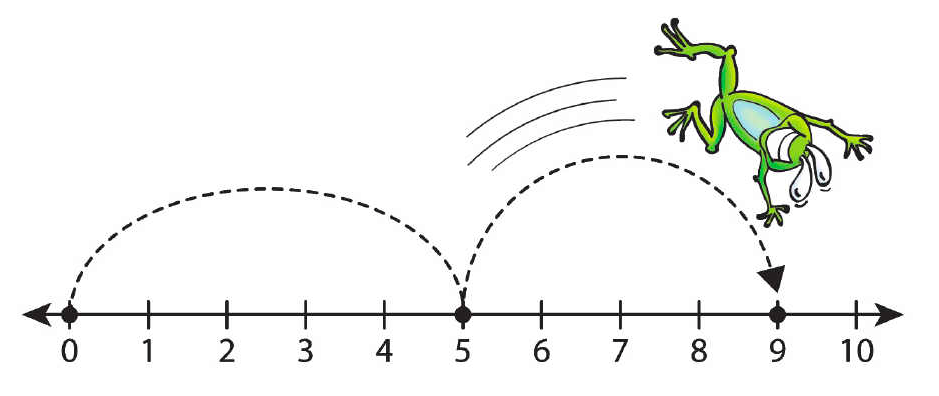
\includegraphics [scale=0.4] {number_line.png} \end{center}
We might simply assume that to every point on the number line there corresponds a rational or irrational number, and that this total collection obeys the same laws of arithmetic as the rational numbers do.

As mentioned above, the need for the real numbers is indicated by empty "holes" in the number line corresponding to the irrational numbers like $\sqrt{2}$.

A problem that arises is how to specify an irrational number non-geometrically and other than as the solution to an equation such as $r^2 = 2$.  In all cases we write particular real numbers as \emph{approximations}.  For example, the square root of $2$ lies between $1$ and $2$ because
\[ 1^2 = 1 < 2, \ \ \ \ 2^2 = 4 > 2 \]
\[ 1.4^2 = 1.96 < 2, \ \ \ \ 1.5^2 = 2.25 > 2 \]
\[ 1.41^2 = 1.9881 < 2, \ \ \ \ 1.42^2 = 2.0164 > 2 \]
at the seventh place
\[ 1.414213^2 = 1.9999984093689998.. < 2 \]
\[ 1.414214^2 = 2.0000012377960004 > 2 \]

and so on.  We can never write down the decimal value of $\sqrt{2}$ exactly, but only approximate it.  The decimal value goes on forever.  

(Because any repeating decimal can be written as a fraction, we know that the sequence cannot repeat).

In a similar way, the number $e$ can be viewed as
\[ \lim_{n \rightarrow \infty} (1 + \frac{1}{n})^n \]

The number $\pi$ can be viewed as the limit of the method of exhaustion applied to the area of a unit circle.

\subsection*{density}

$\circ$  Between any two \emph{real} numbers it is always possible to find a rational number.  
\[ \forall \ a,b \in \mathbb{R} \ \exists \ r \in \mathbb{Q} \ | \ r \in (a,b) \]
Proof:  pick
\[ N \in \mathbb{N} \text{ such that } N > \frac{1}{b-a} \]
Then 
\[ \frac{1}{N} < b - a \]
Let the set 
\[ \mathbf{A} = \{ \ \frac{m}{N}: \ m \in \mathbb{N} \}, \ \ \ \text{a subset of } \mathbb{Q} \]
The claim is that
\[ \mathbf{A} \cap (a,b) \ne \emptyset \]
There do exist numbers within the open interval $(a,b)$ that are in the set $\mathbb{Q}$.

The proof is by contradiction.  Assume on the contrary that the set $\mathbf{A}$ does not contain a rational number lying inside this interval.  In other words:
\[ \mathbf{A} \cap (a,b) = \emptyset \]
Now, find the largest integer $m_1$ such that $m_1/N < a$ (it is OK if $m_1$ is equal to $0$).  Then the next rational number in $\mathbf{A}$ must be larger than $b$ since the set intersection is empty:
\[ \frac{m_1 + 1}{N} > b \]
But this implies that
\[ \frac{m_1 + 1}{N} - \frac{m_1}{N} > b - a \]
\[ \frac{1}{N} > b - a \]
which contradicts our condition on $N$ above.  Hence the assumption is false and so
\[ \mathbf{A} \cap (a,b) \ne \emptyset \]
Thus there must exist a rational number $r$ in $\mathbf{A}$ such that $a < r < b$.

\subsection*{example}
Consider the open interval:  $(\sqrt{2},\sqrt{3})$.  
\[ a = \sqrt{2} \approx 1.414 \]
\[ b = \sqrt{3} \approx 1.732 \]
\[ b-a \approx 0.3178 \]
\[ \frac{1}{b-a} \approx 3.1462 \]
Pick $N \ge 4$, for example
\[ N = 4: \ \ \  1.414 < \frac{6}{4} = 1.5 < 1.732 \]
\[ N = 5: \ \ \  1.414 < \frac{8}{5} = 1.6 < 1.732 \]
\[ N = 6: \ \ \  1.414 < \frac{9}{6} = 1.5 < 1.732 \]
(In this case $N=2$ and $N=3$ happen to work as well).

\subsection*{ordering}
The real numbers can also be ordered.  A simple way is to use the rational numbers as a scaffold or guide.  Recall that we can always find a rational number $r$ that lies in the interval between any two real numbers $a$ and $b$ such that 
\[ r \in (a,b) \]
Then either $a < r < b$ or $b < r < a$ and so
\[ r < b \ \iff \ a < b \]
which orders $a$ and $b$.

Courant and John set up a system in which real numbers are specified as a nested sequence of intervals with rational bounds.
\begin{center} 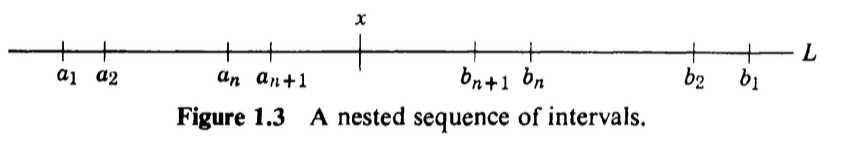
\includegraphics [scale=0.5] {nested_intervals.png} \end{center}
with 
\[ a_1 \le a_2 \le a_3 \le x \le b_3 \le b_2 \le b_1 \]

They say
\begin{quote}let $x$ be confined to a closed interval $I_1 = [a_1,b_1]$ where $a_1$ and $b_1$ are rational.  Within $I_1$ we consider a "subinterval" $I_2 = [a_2,b_2]$ containing $x$, where $a_2$ and $b_2$ are rational.  For example, we may choose for $I_2$ one of the halves of $I_1$, for $x$ must lie in one or both of the halves of $I_1$.  Within $I_2$ we consider a subinterval $I_3 = [a_3,b_3]$ ...  We require that the length of the interval $I_n$ tends to zero with increasing $n$;  that is that the length of $I_n$ is less than any preassigned positive number for all large $n$ ...  A set of closed intervals $I_1, I_2, I_3 \dots$ each containing the next one and such that the lengths tend to zero will be called a "nested sequence of intervals."  The point $x$ is uniquely determined by the nested sequence ... we see that every point $x$, that is, every real number, can be precisely described with the help of infinitely many rational numbers.\end{quote}

Courant
\begin{center} 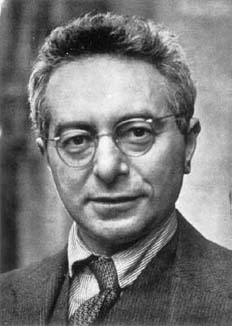
\includegraphics [scale=0.5] {Courant_3.png} \end{center}

The quote above continues:
\begin{quote}As we shall see, this is an \emph{axiom of continuity}:  it guarantees that no gaps exist on the real axis.  We shall use the axiom to characterize the real continuum and to justify all operations with limits which are basic for calculus and analysis.  (There are also many other ways of formulating this axiom ...)\end{quote}

\subsection*{density again}
$\circ$  Between any two rational numbers it is always possible to find a real number.

This is the converse of the statement at the end of the quote.  Courant says it "is not so obvious,;  we shall accept it as a basic axiom."

\[ \forall \ a,b \in \mathbb{Q} \ \exists \ c \in \mathbb{R} \ | \ c \in (a,b) \]

One proof consists of finding a \emph{particular} irrational in the interval $(a,b)$, where $a$ and $b$ are rational.  For $a < b$, we simply add to the number $a$ the following
\[ c = \frac{\sqrt{2}}{2}(b - a) \]
$c$ is smaller than $b - a$ (because $\sqrt{2}/2 < 1$) so the result $a + c$ lies between $a$ and $b$.  We also know that $c$ is irrational, because $\sqrt{2}$ times any rational number is irrational.  Finally, $a + c$ is irrational because adding $\sqrt{2}$ times a rational number to any rational number produces an irrational number.

Proof of the first preliminary requirement:  $\sqrt{2}$ times a rational is irrational.  Suppose for integer $p, q, r, s$ we have
\[ \sqrt{2} \frac{p}{q} = \frac{r}{s} \]
then
\[ \sqrt{2} = \frac{rq}{ps} \]
But the right-hand side is rational, so this is a contradiction.

For the second requirement, again by contradiction suppose
\[ \sqrt{2} \ \frac{p}{q} +  \frac{s}{t} = \frac{u}{v} \]
for integer $p, q, r, s, u, v$.  But the right-hand side of
\[ \sqrt{2} = \frac{q}{p} ( \frac{u}{v} - \frac{s}{t}) \]
is rational, so this is a contradiction.

Note that powers are different.  What do you think about
\[ r = \sqrt{2}^{\sqrt{2}} \]
You may think $r$ is "likely" to be irrational.  Just a mess.  But how about
\[ r^{\sqrt{2}} \]
Whether $r$ is rational or irrational
\[ r^{\sqrt{2}} = (\sqrt{2}^{\sqrt{2}})^{\sqrt{2}} = \sqrt{2}^2 = 2 \]
!!

$\circ$  Between any two real numbers it is always possible to find another real number.  
\[ \forall \ a,b \in \mathbb{R} \ \exists \ c \in \mathbb{R} \ | \ c \in (a,b) \]

This one is subtle.  Suppose the two real numbers are "really, really close."  

We suppose that they are not equal, so they must be different, say $a < b$.

Since they are different, at some stage in the decimal expansions of $a$ and $b$, there must be a first position at which $a$ and $b$ differ.  If $b$ does not have a $0$ at the next position, terminate there and that will be $c$.

For example:
\[ a = 1.23456789129.. \]
\[ b = 1.23456789133.. \]
\[ c = 1.23456789130.. \]

$b$ must have some digit following this first position where it does not match $a$, and which is also not equal to zero (otherwise it would be a terminating decimal and thus a rational number).  So we can always find a place to terminate to form $c$.

\textbf{Eternity is a very long time, especially towards the end. }

(credited to Woody Allen)

\subsection*{infinity}

The supply of integers or even natural numbers $\mathbb{N}$ is infinite, because if not, then there would be a maximum integer $m \in \mathbb{N}$.  But $m + 1$ is also $\in \mathbb{N}$, and $m+1 > m$, which is a contradiction.

Both the real numbers and the rational numbers also come in an infinite supply, for basically the same reason.  Just add $1$ to the "maximum" $m$, then find a real or a rational in the interval $(m,m+1)$.  

Even for a finite interval such as $(0,1)$, the properties described above prove that this finite interval contains an infinite number of both rational and real numbers.

But more than this, in an important sense, there are \emph{many more} real numbers than rational numbers.

The idea of the proof is to show that one can set up a correspondence between $\mathbb{N}$ and $\mathbb{Q}$, assigning each number $r \in \mathbb{Q}$ in a particular order to $1,2,3, \dots$.  Here is the figure from Courant and John:
\begin{center} 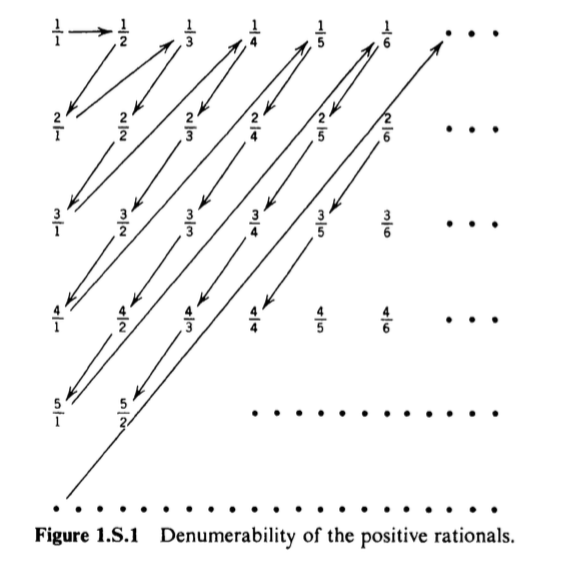
\includegraphics [scale=0.6] {denumerability.png} \end{center}

We first set up the sequence
\[ \frac{1}{1} \ \ \ \frac{1}{2}, \frac{2}{1} \ \ \  \frac{1}{3}, \frac{2}{2}, \frac{3}{1} \ \ \ \frac{1}{4}, \frac{2}{3}, \frac{3}{2}, \frac{4}{1} \ \ \ \frac{1}{5}, \frac{2}{4}, \frac{3}{3}, \frac{4}{2}, \frac{5}{1} \ \ \  \frac{1}{6}, \frac{2}{5}, \frac{3}{4}, \frac{4}{3}, \frac{5}{2}, \frac{6}{1} \dots \]
Then we remove all fractions that are duplicates by way of not being in lowest terms.
\[ \frac{1}{1} \ \ \ \frac{1}{2}, \frac{2}{1} \ \ \  \frac{1}{3}, \frac{3}{1} \ \ \ \frac{1}{4}, \frac{2}{3}, \frac{3}{2}, \frac{4}{1} \ \ \ \frac{1}{5}, \frac{5}{1} \ \ \  \frac{1}{6}, \frac{2}{5}, \frac{3}{4}, \frac{4}{3}, \frac{5}{2}, \frac{6}{1} \dots \]

Finally, each $r$ in this sequence is assigned to a natural number (in the sequence $\mathbb{N}$), establishing the denumerability property.

Cantor showed that such a correspondence is impossible for $\mathbb{R}$.  The proof of this is is not hard, but we will skip it here.  You can check out the chapters on Georg Cantor in Dunham's \emph{Journey Through Genius}.

Thus, the rational numbers are said to be "countably infinite", while the real numbers are not countable.  (There is also a proof that the transcendental numbers are much more numerous than the non-transcendental ones).

\subsection*{Completeness axiom}
Suppose $\mathbf{S}$ is a non-empty set of real numbers and suppose there is a real number $B$ such that $B$ is greater than or equal to every member of $\mathbf{S}$:
\[ \forall \ x \in \mathbf{S}, x \le B \]

$\circ$  We say that the number $B$ is an \emph{upper bound} for $\mathbf{S}$;   $\mathbf{S}$ is \emph{bounded above} by $B$.  

$\circ$  The alternative is that the set $\mathbf{S}$ is not bounded above.  An example might be $[1,\infty)$.

$\circ$  If a set has at least one $B$, it will have many upper bounds, because there are many real numbers  $x > B$.

$\circ$  $B$ may or may not be $\in \mathbf{S}$.  If it is, then $B$ is the largest or maximum element of $\mathbf{S}$.  There can be at most one such $B$.

\subsection*{examples}
For the set of all real $x$ in $[0,1)$ (i.e. $0 \le x < 1$), the set is bounded above by $1$ and but it has no maximum element.  We say that $\sup(\mathbf{S}) = 1$.  ($\sup$ is for "supremum").

For the set of all real $x$ in $[0,1]$ (i.e. $0 \le x \le 1$), the set is bounded above by $1$ and $1$ is the maximum element of the set.  We say that $\max(\mathbf{S}) = 1$.  If $\mathbf{S}$ contains a greatest element, then that element may also be called the supremum.

For sets like the first one we basically use the concept of the \emph{least upper bound} in place of the maximum element.

$\circ$  A number $B$ is called the least upper bound of a non-empty set $\mathbf{S}$ if $B$ is an upper bound for $\mathbf{S}$ and no number less than $B$ is an upper bound for $\mathbf{S}$.

$\circ$  The completeness axiom says that any non-empty set $\mathbf{S}$ of real numbers which is bounded above has a supremum;  i.e. there is a real number $B$ such that $B = \sup(\mathbf{S})$.

It all sounds very complicated but there are only three cases for the set $\mathbf{S}$:  it is not bounded above and "extends" to infinity, it is bounded above and the least upper bound is $\in \mathbf{S}$, it is bounded above and the least upper bound $B$ is not $\in \mathbf{S}$.  We call $B$ the supremum.

\subsection*{Completeness Axiom}
Every nonempty subset of $\mathbb{R}$ that is bounded above has a supremum in $\mathbb{R}$

\begin{quote}The completeness axiom captures the distinction between the reals and the rationals.  Replacing $\mathbb{R}$ with $\mathbb{Q}$ in this axiom gives a statement that isn't true.\end{quote}

The set $\{ x \in \mathbb{Q} \ | \ x^2 < 2 \}$ has a supremum ($\sqrt{2}$) but that number is only in $\mathbb{R}$ and not in $\mathbb{Q}$.

\subsection*{Archimedean property}
$\circ$  For every real $x$ there exists a positive integer $n$ such that $n > x$.

$\circ$ If $x > 0$ and if $y$ is an arbitrary real number, then there exists a positive integer $n$ such that $nx > y$.  Proof:  apply the previous theorem with $x$ replaced by $y/x$.

\begin{quote}The property described is called the Archimedean property of the real- number system.  Geometrically it means that any line segment, no matter how long, may be covered by a finite number of line segments of a given positive length, no matter how small. In other words, a small ruler used often enough can measure arbitrarily large distances. Archimedes realized that this was a fundamental property of the straight line and stated it explicitly as one of the axioms of geometry.  ---Apostol\end{quote}

Apostol
\begin{center} 
\includegraphics [scale=0.4] {Apostol.png} \end{center}

$\circ$ If three real numbers $a,y,$ and $y$ satisfy
\[ a \le x \le a + \frac{y}{n} \]
for every integer $n \ge 1$, then $x = a$.

Proof:  By the Archimedean property, if $x > a$ then there is a positive integer such that $n(x-a) > y$ but this contradicts the statement $x \le a + y/n$.  Hence $x = a$.

\section*{Limits}
At this point we will start talking about limits, which are the basis of calculus.

Consider the graph of a function of $x$, call it $f(x)$.  We might choose a power of $x$ similar to $y = x^2$ or $y = x^3 - x$, which affirmatively has two properties that are of interest here:  continuity and differentiability.
\begin{center} 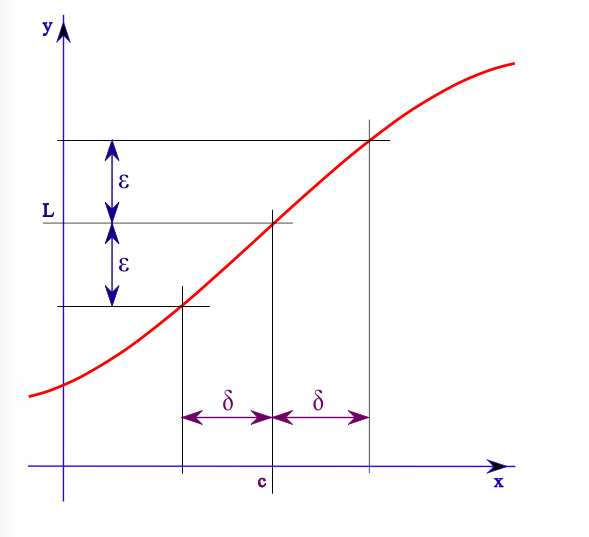
\includegraphics [scale=0.5] {epsilon-delta.png} \end{center}
We focus on the neighborhood of a point on the $x$-axis, $x=c$.

By inspection of the graph we see that the value of $f(x)$ at $c$ is equal to $L$, and furthermore, for points near $c$, the value of $f$ at those points is not too different from $L$.

We would like to say that the \emph{limit} of $f(x)$ as $x$ \emph{approaches} $c$ is equal to $L$.  The idea is that we can make $f(x)$ as close to $L$ as we please, provided we choose $x$ sufficiently close to $c$.

\begin{quote}When the values successively attributed to a variable approach indefinitely to a fixed value, in a manner so as to end by differing from it by as little as one wishes, this last is called the limit of all the others.  ---Cauchy\end{quote}

\begin{center} 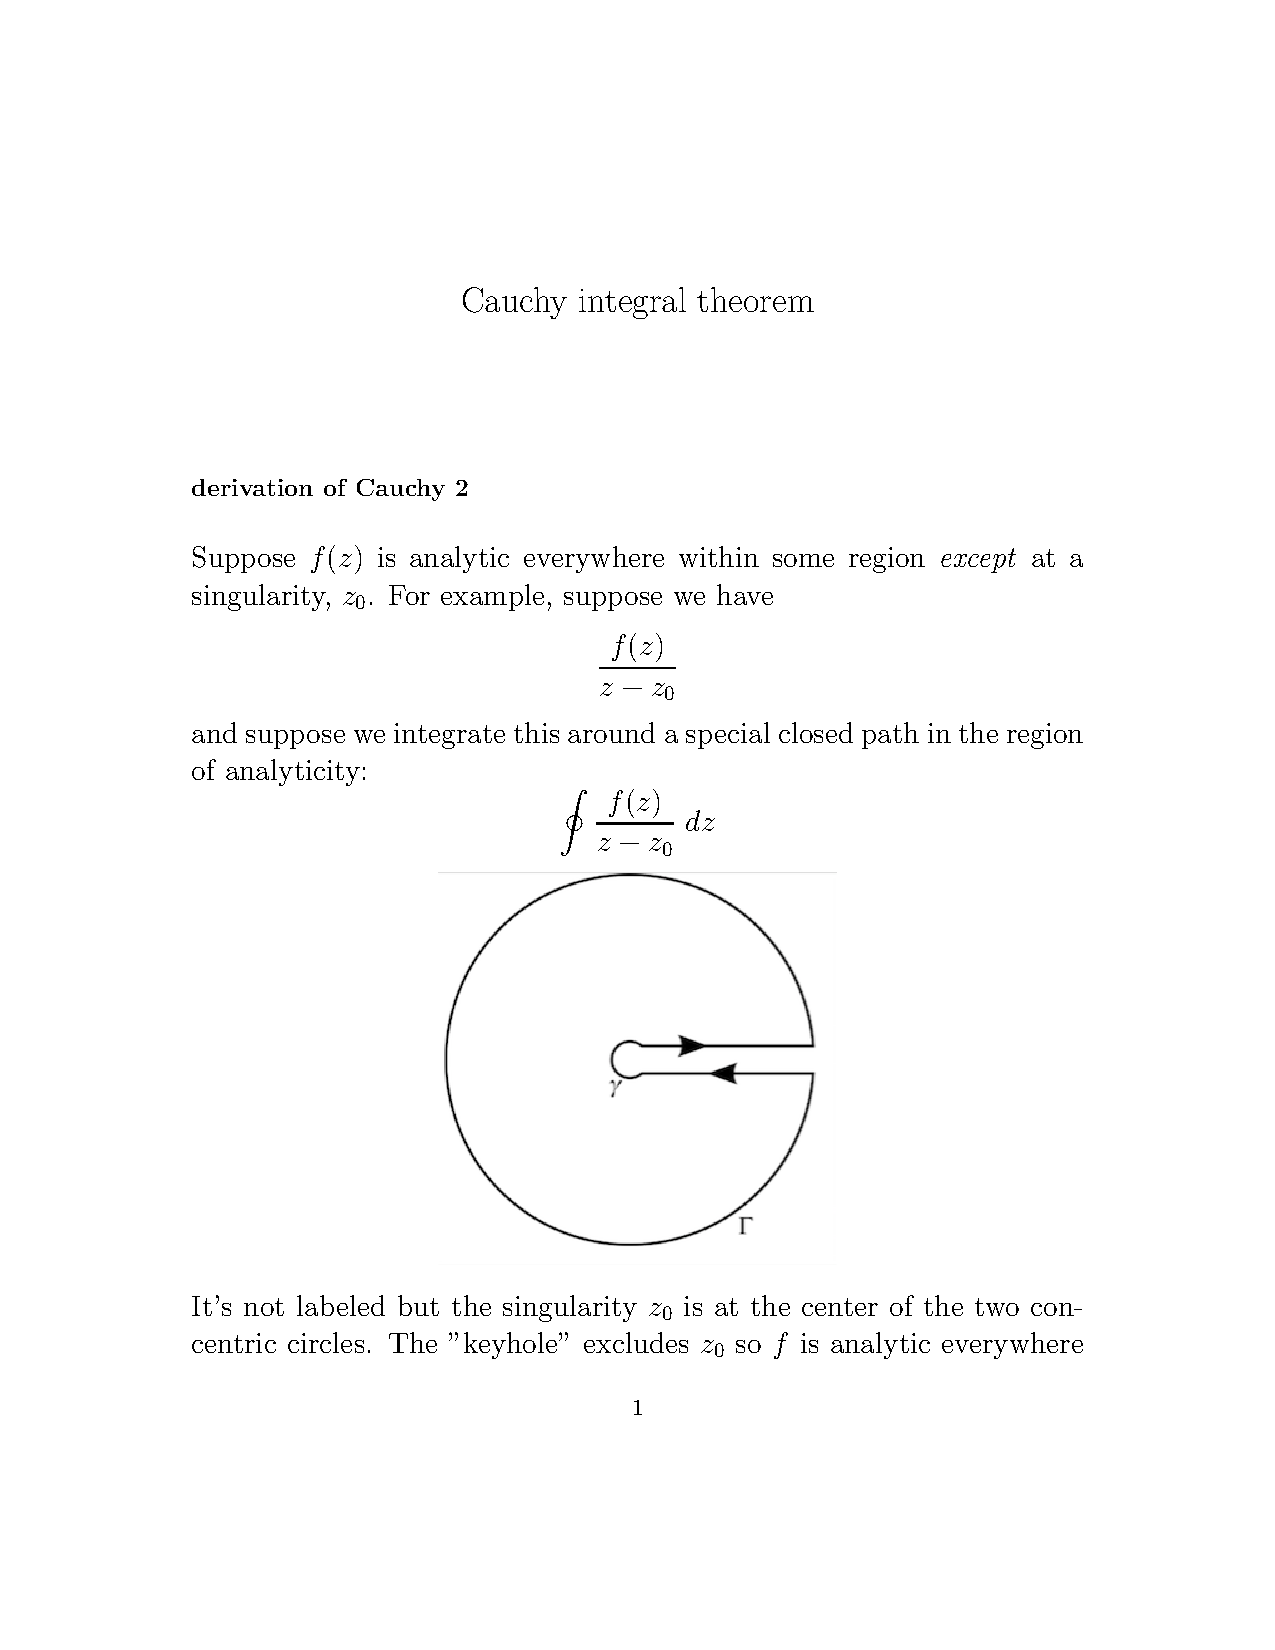
\includegraphics [scale=0.3] {Cauchy} \end{center}

Modern mathematicians don't like that word "approach", which conjures up movement and the involvement of time, and they don't like reasoning from what they see in a graph, in part because no graph can show the whole function for the general case.  Instead we will use an algebraic method from the formal apparatus of calculus.

There are two equivalent approaches, neighborhoods, and epsilon-delta formalism.  Let's look at neighborhoods briefly first.
\subsection*{neighborhoods}

First, an \emph{interval} between two real numbers $a$ and $b$ ($a < b$) contains every real number $a < x < b$.
\[ (a,b) = x \ | \ a < x < b \]
The "$|$" means $x$ "such that" the condition $a < x < b$ holds.  (We rely on your intuition about what a real number is for now but will have much more to say later as well).

A \emph{closed} interval $[a,b]$ includes the endpoints ($a \le x \le b$), while an \emph{open} interval $(a,b)$ excludes them.  Half-open intervals like $[a,b)$ may be defined, and an interval with $\pm \ \infty$ as an endpoint is always open on that end, for example:  $[a,\infty)$.

Any open interval with a point $p$ as its midpoint is called a \emph{neighborhood} of $p$.  The distance $r$ from $p$ to the boundary of a particular neighborhood may be large or very very small.  We denote a neighborhood of $p$ as $N(p)$.
\[ N(p) = x \ \text{ such that } \ |x-p| < r \].

To say that the limit $f(x) \rightarrow L$ exists, we mean that for every neighborhood $N_1(L)$, there exists some neighborhood $N_2(p)$ such that $f(x) \in N_1(L)$ whenever $x \in N_2(p)$.  We exclude the point $x = p$.

The idea of a neighborhood is a nice abstraction to hide the apparatus of modern calculus, which we look at next.
\begin{center} 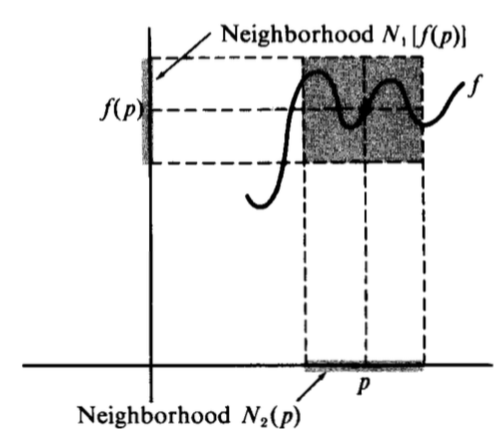
\includegraphics [scale=0.4] {neighborhood.png} \end{center}

\subsection*{epsilon-delta game}
The formal method uses numbers called $\epsilon$ and $\delta$ and is originally due to Bolzano.

We say that, \emph{if} for all points $x$ within a specified distance $\delta$ of $c$, we find that $f(x)$ lies within a specified distance $\epsilon$ from $L$, \emph{then} the limit is $L$.

To do this we must choose $\epsilon$ first.  That's why I call it a game.  Why don't you go first?  Choose $\epsilon$, which provides a constraint on how close to $L$ you want the value of $f(x)$ to be:  you require that  $|f(x) - L| < \epsilon$.  The \emph{distance} from $f(x)$ to $L$ must be less than $\epsilon$.

Now that I know your $\epsilon$, I must try to find a suitable $\delta$.  If I can, then you get another chance, and will presumably choose a smaller $\epsilon$.  

If I can show that it is possible to find a $\delta$ to guarantee that your constraint is satisfied for \emph{all} values of $\epsilon > 0$ \emph{no matter how small}, then I win and the limit exists.  If not, it doesn't.

Here is a formal definition:
\[ \forall \ \epsilon > 0, \exists \ \delta > 0 \ | \ \forall \ x, \ 0 < | x - c| < \delta \rightarrow | f(x) - L | < \epsilon \]

$\circ$  for \emph{any} real number epsilon $\epsilon > 0$

$\circ$  there exists (we can find) a real number delta $\delta > 0$ 

$\circ$  such that for all $x$

$\circ$  if c - $\delta < x  < c + \delta \ \ \ (c > 0)$

$\circ$  then $f(x) - \epsilon < L  < f(x) + \epsilon \ \ \ (f(x) > 0)$

In this figure (from Courant and John), the mapping from $x$ to $y = f(x)$ is depicted generally using two number lines.
\begin{center} 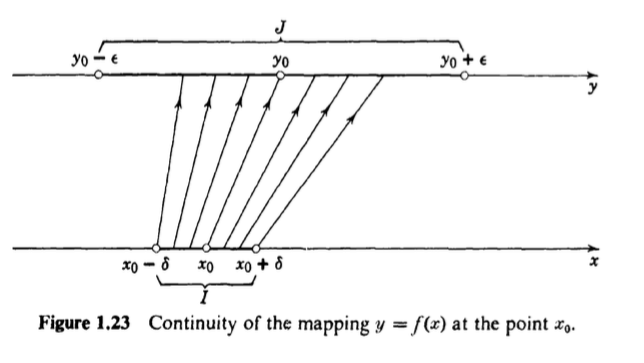
\includegraphics [scale=0.6] {continuity.png} \end{center}
(This figure talks about continuity, which we will come to in a minute).

\subsection*{more}
We describe the limit defined above by saying that
\[ \lim_{x \rightarrow c} f(x) = L \]

The limit as $x$ tends to, or approaches, $c$ is equal to $L$.

Important points about limits:

$\circ$  We do not require that $f(c) = L$.

The function $f(x)$ may or \emph{may not} have the value $L$ at $x=c$ and the limit can still exist and be equal to $L$.  Suppose we have $f(x) = x$, whose graph is the line $y=x$, except that we decide to define $f(0) = 1$, leaving a hole in our line $y=x$ at the point where $x=0$.  The limit of $f(x)$ at $x=0$ is equal to $0$, despite the fact that $f(0) = 1$.

Alternatively, suppose that we only allow values of $x$ in the open interval $(a,b)$, and the limit $x \rightarrow a +$ (from the right) does exist.  Since we have restricted the domain of $f$ to values $x > a$ the limit $x \rightarrow a -$ certainly does not exist, and in fact the left-hand endpoint $a$ is not in the domain of $f$.

We say that such a limit ($x \rightarrow a +$) is a \emph{one-sided} limit.  If the two one-sided limits do not agree at a particular value of $c$, then the (two-sided) limit does not exist.

$\circ$  We allow the existence of a limit as $x$ approaches $\infty$
\[ \lim_{x \rightarrow \infty} f(x) = L \]
To define this limit, play the epsilon-delta game (typically, using $c$ instead of $\delta$) and say that if, when $x > c$, $|f(x) - L| < \epsilon$, the limit "at" $\infty$, or as $x$ \emph{tends to} $\infty$, exists and has the value $L$.

\subsection*{example:  floor}
Consider the "floor" function, which is defined on the real numbers and has the value of the largest integer less than or equal to $x$.
\begin{center} 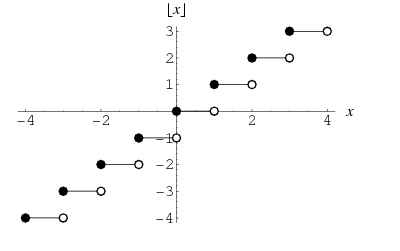
\includegraphics [scale=0.75] {floor.png} \end{center}
The floor function has one-sided limits (from the right) at integral values of $x$, but the limit at $x=2$, for example, does not exist, because those two one-sided limits are not the same.

\subsection*{example:  inverse}
Consider the function $f(x) = 1/x$.  This function is undefined at $x=0$ since division by zero is not defined.  As $x$ gets close to zero from the right, $1/x$ takes on larger and larger positive values.

Some people will say that limits can have infinite values.  In the case of $f(x) = 1/x$, informally, we accept that the limit as $x \rightarrow 0+$ exists and has the value $\infty$.  Speaking more formally, we might say that the function "diverges" or "grows without bound".

In any case since for $f(x) = 1/x$
\[ \lim_{x \rightarrow 0+} \ne \lim_{x \rightarrow 0-} \]
so the limit as $x \rightarrow 0$ does not exist (abbreviated D.N.E.).

\subsection*{example:  sine of 1/x}
The trigonometric functions sine and cosine are, of course, periodic.  For any value of $\theta$
\[ \sin \theta = \sin ( \theta \pm 2 \pi) \]
The maximum values of the sine function (for $\theta > 0$) occur at
\[ \theta = \frac{\pi}{2},  \frac{5\pi}{2}, \frac{9\pi}{2}, \frac{13\pi}{2} \dots \]
The corresponding maximum values of $\theta = 1/x$ occur at
\[ x = \frac{2}{\pi}, \frac{2}{5 \pi}, \frac{2}{9 \pi}, \frac{2}{13 \pi} \dots \]
The corresponding decimal values are approximately
\[ x = 0.6366, 0.1273, 0.0707, 0.0490 \]
As $\pi/2 + 2k\pi$ gets larger, the corresponding values for the inverse get smaller, and more closely spaced together.

Now, $1/x$ grows without bound as $x \rightarrow 0$.  This means that there is an infinite number of places where the value of the function $\sin(1/x)$ is equal to $1$ and indeed, takes on all possible values in its range $[-1,1]$, and this occurs more and more rapidly as $x \rightarrow 0$.

In short, the value oscillates and does so more extremely the closer $x \rightarrow 0$.
\begin{center} 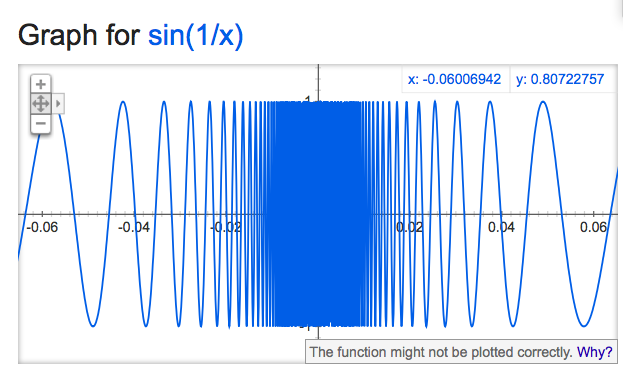
\includegraphics [scale=0.4] {sinxinverse.png} \end{center}
The limit as $x \rightarrow 0$ D.N.E.

\subsection*{triangle inequality:  geometric}
We want to develop a proof of the sum rule and the product rule for limits.  To do that, we will first need something called the triangle inequality, which says that
\[ |a + b| \le |a| + |b| \]

It is called the triangle inequality because the version from geometry says that the combined lengths of any two sides of a triangle are greater than the length of the third side.
\begin{center} 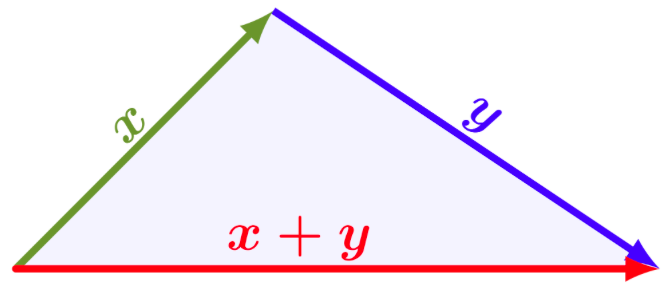
\includegraphics [scale=0.4] {triangle_inequality.png} \end{center}
The geometric version is pretty obvious.  The equals part is for the case when the triangle collapses to a straight line.

Recall that the absolute value or modulus function is
\[ f(x) = |x| =
\begin{cases}
\ \ x, \ \ \ x \ge 0 \\
-x, \ \ \ x < 0
\end{cases}
\]

Going back to the triangle inequality
\[ |a + b| \le |a| + |b| \]
there are 3 cases.  

The first case is that both $a \ge 0$ and $b \ge 0$.  In terms of the number line, we move right a distance $a$, and then we move further right a distance $b$.  The total distance from the origin is $a + b$.

Formally if $a \ge 0$ and $b \ge 0$ then
\[ a + b \ge 0 \]
Since for $x \ge 0$, $|x| = x$, we have
\[ |a+b| = a + b \]
\[ = |a| + |b| \]

Alternatively both values are less than zero.  In terms of the number line, everything is the same except we move to the left from the origin.  The total distance from the origin is then $|a + b|$.

Formally, write this using $c = -a$ and $d = -b$.  Then
\[ |a| + |b| = |-c| + |-d| = c + d = |-(c+d)| = |a + b| \]
and we still have equality.

The third case is that one value is positive and one is negative in which case the sum $|a+b|$ is smaller than the larger of $|a|$ or $|b|$ and the inequality is true.

For the more formal proof (especially for the third case), we follow Apostol.  A preliminary theorem is that given $a \ge 0$
\[ |x| \le a \iff -a \le x \le a \]

We use this theorem often in calculus:  thinking about an interval with endpoints a distance $a$ from a central point $p$, then the 
\[ |x - p| < a \iff  -a < x - p < a \]

Theorem:
\[ |x| \le a \iff -a \le x \le a \]

Proof in the forward direction:  suppose $|x| \le a$ (with $a \ge 0$).  

Then by adding $-a$ and $- |x|$ to both sides, we also have $-a \le - |x|$.

But either $x = |x|$ or $x = -|x|$ and so
\[ -|x| \le x \le |x| \]
Putting it all together
 $-a \le -|x| \le x \le |x| \le a$.  This proves the statement.

To prove the converse, assume $-a \le x \le a$.

Then if $x \ge 0$ we have $|x| = x \le a$, whereas if $x \le 0$ we have $|x| = - x \le a$.  In either case we have $|x| \le a$, and this completes the proof.

Now to get the triangle inequality theorem, add the two inequalities 
\[ - |x| \le x \le |x| \]
\[ - |y| \le y \le |y| \]
we obtain
\[ - ( |x| +  |y| ) \le x + y \le ( |x| + |y| ) \]

The above statement is equivalent to the right hand side of the previous theorem (with $a = |x| + |y|$ and $x$ for $x+y$)
\[ |x| \le a \iff -a \le x \le a \]

Therefore the left hand side is also true:
\[ | x+y | \le |x| + |y| \]
This proves the triangle inequality.

\subsection*{proof of the sum rule for limits}
Assume that
\[ \lim_{x \rightarrow c} f(x) = L \]
\[ \lim_{x \rightarrow c} g(x) = M \]

We want to show that
\[ \lim_{x \rightarrow c} f(x) + g(x) = L + M \]
The limit of the sum is the sum of the limits.

Let $\epsilon > 0$ be arbitrary.

Then the existence of the limits means that
\[ \forall \ \epsilon, \exists \ \delta_1 > 0 \ | \ \forall \ x, \ 0 < | x - c| < \delta_1 \rightarrow | f(x) - L | < \epsilon/2 \]
and
\[ \forall \ \epsilon, \exists \ \delta_2 > 0 \ | \ \forall \ x, \ 0 < | x - c| < \delta_2 \rightarrow | g(x) - M | < \epsilon/2 \]
Let
\[ \delta = \text{ min } (\delta_1, \delta_2) \]
Now for $|f(x) < \delta|$
\[ | f(x) - L + g(x) - M| < \epsilon \]
But by the triangle inequality the left-hand side is 
\[   | f(x) - L| + |g(x) - M| < \epsilon \]
which proves the theorem.
(Needs work).

\subsection*{proof of the product rule for limits}
Assume that
\[ \lim_{x \rightarrow c} f(x) = L \]
\[ \lim_{x \rightarrow c} g(x) = M \]

We want to show that
\[ \lim_{x \rightarrow c} f(x) \cdot g(x) = LM \]
The limit of the product is the product of the limits.

Now we will assume that
\[ \lim_{x \rightarrow c} f(x) \cdot g(x) = \lim_{x \rightarrow c} f(x) \cdot \lim_{x \rightarrow c} g(x) \]
(with the proviso that the limits on the right hand side are known to exist and are finite.  This is a bit too subtle at the moment).

We need to show that
\[ f(x) \cdot g(x) - LM \]
is small.  Subtract $L g(x)$ and add it back
\[ f(x) \cdot g(x) - LM = f(x) \cdot g(x) - L g(x) + L g(x) - LM \]
\[ f(x) \cdot g(x) - LM = (f(x) - L) g(x) + L (g(x) - M ) \]
Take absolute values
\[ |f(x) \cdot g(x) - LM| = |(f(x) - L) g(x) + L (g(x) - M )| \]
Use the triangle inequality
\[ |f(x) \cdot g(x) - LM| \le |(f(x) - L) g(x)| + |L (g(x) - M )| \]
\[ |f(x) \cdot g(x) - LM| \le |(f(x) - L) | | g(x) | + | L | | (g(x) - M )| \]

Now, play the epsilon-delta game:  you pick $\epsilon$ and then I concentrate on a region so close to $c$ that
\[ |f(x) - L | < \epsilon \]
and
\[ |g(x) - M | < \epsilon \]
(if your epsilon is too large I will pick $|g(x) - M < 1|$ so this inequality is true no matter what $\epsilon$ is.

Then I have
\[ |f(x) - L | < \epsilon \]
\[ |g(x) - M | < \epsilon \]
\[ |g(x) < |M| + 1 \]

Go back to the equation we obtained above
\[ |f(x) \cdot g(x) - LM| \le |(f(x) - L) | | g(x)| + | L | | (g(x) - M )| \]
substitute
\[ |f(x) \cdot g(x) - LM| < \epsilon \ (|M| + 1) + | L | \ \epsilon \]
\[ < \epsilon \ (|M| + |L| + 1) \]

as Adrian Banner says in \emph{Calculus Lifesaver}:

\begin{quote}
That's almost what I want!  I was supposed to get $\epsilon$ on the right-hand side, but I got an extra factor of $|M| + |L| + 1$.  This is no problem---you just have to allow me to make my move again, but this time I'll make sure that $|f(x) - L|$ is no more than $\epsilon/(|M| + |L| + 1)$, and similarly for $|g(x) - M|$.  Then when I replay all the steps, $\epsilon$ will be replaced by $\epsilon/(|M| + |L| + 1)$, and at the very last step, the factor $|M| + |L| + 1$ will cancel out and we'll just get our $\epsilon$.  So we have proved the result.
\end{quote}

\section*{Continuity}
Continuity has an intuitive definition:  if we can graph a function \emph{without lifting our pencil from the paper}, then the function is continuous.

Here are some graphs showing examples of how continuity can fail.
\begin{center} 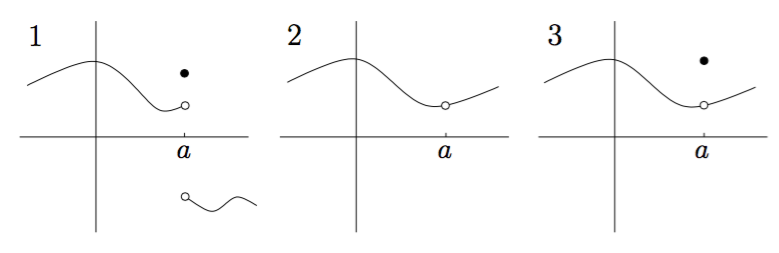
\includegraphics [scale=0.5] {continuity_failure.png} \end{center}
\begin{center} 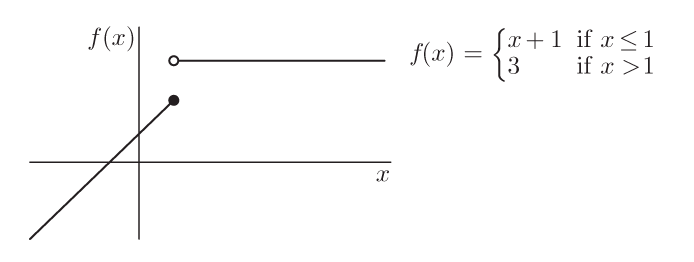
\includegraphics [scale=0.5] {continuity_failure2.png} \end{center}

For a function to be continuous at a point $x=c$, we imagine that if we vary $x$ in neighborhood of $c$, then $f(x)$ should not change in value by too much.

Again, we will call that value $L$, the limit of $f(x)$ as $x \rightarrow c$.  For $L$ to exist we require that the two one-sided limits be equal.  

In addition, it must also be true that $f(c) = L$.

\subsection*{fancy definition}
If we had not previously developed the concept of a limit, we might proceed as follows:  a function $f : \mathbb{R} \rightarrow \mathbb{R}$ is continuous at $c \in \mathbb{R}$ if and only if
\[ \forall \ \epsilon > 0 \ \exists \ \delta > 0 \ \text{ such that, if } |x-c| < \delta, \text{ then } |f(x) - f(c)| < \epsilon \]

\subsection*{example:  absolute value}
An algebraic definition of the absolute value function is piecewise:
\[ |x| =
\begin{cases}
\ \ x, \ \ \ x \ge 0  \\
-x, \ \ \ x < 0
\end{cases}
\]
\begin{center} 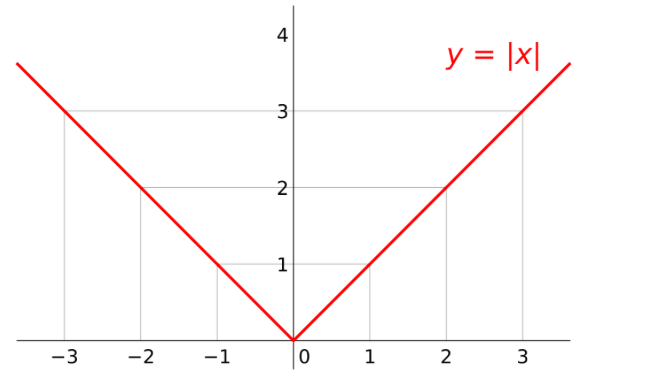
\includegraphics [scale=0.4] {abs.png} \end{center}
The function $f(x) = |x|$ is continuous at $x=0$ because the two one-sided limits exist and are equal to each other.  They are also equal to $f(0) = 0$.

\subsection*{example:  constant}
Suppose $f(x) = a$ for some real number $a$.  Then no matter what $\epsilon$ is chosen and no matter what real number $c$ is chosen
\[ f(x) = f(c) = a \]
so
\[ |f(x) - f(c)| < \epsilon \]

\subsection*{example:  x}
Suppose $f(x) = x$.  
\[ \lim_{x \rightarrow c} f(x) = c  = f(c) \]
so $f$ is continuous at $c$.

Or choose $\delta = \epsilon$.  Then, if $|x-c| < \delta$
\[ c- \delta < x < c + \delta \]
\[ f(x) = x \]
\[ f(x) - c < \delta = \epsilon \]
\[ | f(x) - c | < \epsilon \]
so $f$ is continuous at $c$

\subsection*{example:  constant factor}
Suppose $f(x) = cx$ ($c \in \mathbb{R}$).  Use the $\epsilon-\delta$ game to prove that $f$ is continuous.

Proof:  the function "stretches" $x$ by a factor of $c$.  Hence $\delta$ will also be stretched.  Set $\delta = \epsilon/c$.  Then, if $|x-a| < \delta$ we have
\[ |f(x) - f(a)| = |cx - ca| = c |x-a| < c \delta = c \epsilon / c = \epsilon \]
Hence $f$ is continuous at every $a \in \mathbb{R}$.

\subsection*{example:  product rule}
How to prove that $f(x) = x^2$ is continuous?  One way is to try adjusting $\delta$ based on the value of $a$ (e.g. min $(| \sqrt{a^2 + \epsilon} \ \pm a|)$), but a better way is to invoke the product rule.

If $f: \mathbb{R} \rightarrow \mathbb{R}$ and $g: \mathbb{R} \rightarrow \mathbb{R}$ are both continuous at $a \in  \mathbb{R}$, then $fg$ is continuous at $a$.

First, prove $f(x) = x$ is continuous.  Then define $f(x) = g(x) = x$.  So $x^2 = f(x) g(x)$ in continuous.

By induction then, all powers $f(x) = x^n$ are continuous.

\subsection*{proof of the product rule for continuity}
Let $f$ and $g$ be functions defined on an open subset of $\mathbb{R}$.  We have that $f$ and $g$ are both continuous at $c$ which means that
\[ \lim_{x \rightarrow c} f(x) = L \]
\[ \lim_{x \rightarrow c} g(x) = M \]
Then
\[ \lim_{x \rightarrow c} f(x) \cdot g(x) = \lim_{x \rightarrow c} f(x) \cdot \lim_{x \rightarrow c} g(x) = LM \]

To obtain this result we have used the product rule for limits. 

\subsection*{example:  inverse}
Consider the function $f(x) = 1/x$.  Above we pointed out that this function is undefined at $x=0$ since division by zero is not defined.  But there is nothing to stop us from defining the function piecewise, like so:

\[ f(x) = 
\begin{cases}
\frac{1}{x} \ \ x \ne 0 \\
0 \ \ x = 0 
\end{cases} \]

As $x$ gets close to zero from the right, $1/x$ continues to take on larger and larger positive values, but then dives to $0$ at $x=0$ and then further dives toward $-\infty$ as we pass to the left of zero.

Trick question:  give an example of a function $f : \mathbb{R} \rightarrow \mathbb{R}$ that is not continuous at zero.  If you said the inverse, that is not correct.  The reason is that the inverse is not $f : \mathbb{R} \rightarrow \mathbb{R}$ because \emph{it is not defined at zero}.

On the other hand, $f(x) = \sin(x)$ \emph{is} $f : \mathbb{R} \rightarrow \mathbb{R}$ even though the values actually output by the function are $f(x) \in [-1,1]$.  That interval is the \emph{image} of the function, any codomain so that the image is contained in the codomain will do.

\subsection*{example}
A famous (but weird) function is defined as
\[ f(x) =
\begin{cases}
1 \ \ \text{ if } x \in \mathbb{Q} \\
0 \ \ \text{ if } x \notin \mathbb{Q} 
\end{cases}
\]

As we said before, you can imagine that the graph of this function looks like a linear hairbrush, with spikes at each rational number.

However, any interval such as $[0,1]$, or $[0.001, 0.002]$ contains an infinite number of rational numbers, but an even larger infinite number of real numbers.  In other words, we only get the hairbrush image if we exclude denominators greater than some value.  And we get the exact same image if we blow up any portion of the graph.

This is hard to think about.

The first function is not continuous anywhere, but the following variant is:
\[ f(x) =
\begin{cases}
x \ \ \text{ if } x \in \mathbb{Q} \\
0 \ \ \text{ if } x \notin \mathbb{Q} 
\end{cases}
\]

Why?

\subsection*{uniform continuity}
The notion of continuity described so far is called "pointwise."  We first pick a point $c$, and then working near that point, we pick an $\epsilon$ and then a $\delta$ and so on.  A particular $\delta$ may be satisfactory for some values of $c$ and not for others.

One can pick a "one-size-fits-all" $\delta$ for some functions and intervals, but not always.  

Weierstrass and his student Heine developed the idea of "uniform continuity".

\begin{center} 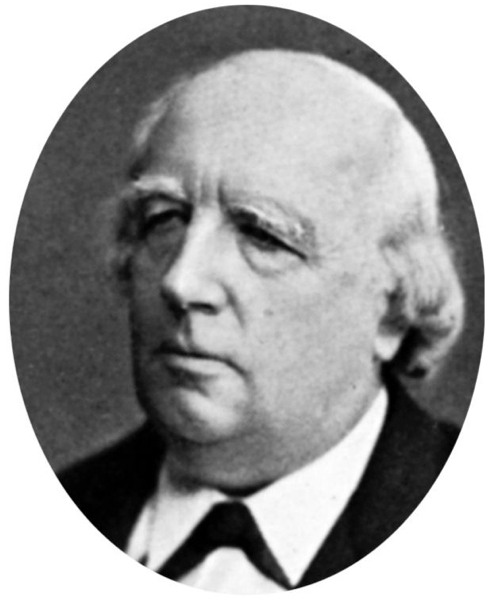
\includegraphics [scale=0.4] {Weierstrass} \end{center}
Weierstrass

A function $f$ is uniformly continuous on some domain if, for every $\epsilon > 0$, there exists a $\delta > 0$ so that, if $x$ and $y$ are any two points in the domain within $\delta$ units of one another, then $|f(x) - f(y)| < \epsilon$.  This $\delta$ must work everywhere in the domain.

It turns out that a function can be pointwise- by not uniformly continuous.  Consider $f(x) = 1/x$ on the open interval $(0,1)$.  The problem is that the values of the function rise to $\infty$ as $x \rightarrow 0$.  Suppose you have some $\delta$ that works for a particular $\epsilon$ near point $c$.  We can always move far enough to the left to a new pair $x,y$ so that the rise in $f(x)$ for a change in $x$ of $\delta$ is $> \epsilon$.

However, Heine proved that a function continous on a closed, bounded interval $[a,b]$ must by uniformly continuous.  According to the internet, 
"a function is uniformly continuous on $(0,1)$ if and only if it can be extended continuously to $[0,1]$."

\section*{Differentiability}
We find the derivative of a simple function as the difference quotient.  

Suppose we have $y=f(x)$ and we are on the graph of the function $f$ at the point $(x,y)$.  Move a little bit to the right, staying on the graph, and now $y + \Delta y = f(x + \Delta x)$.  Then the change in $y$ is
\[ \Delta y = f(x + \Delta x) - f(x) \]
and the slope of the line between these two points is
\[ \frac{\Delta y}{\Delta x} = \frac{f(x + \Delta x) - f(x)}{\Delta x} \]
while I usually write more simply as
\[  \frac{f(x+h) - f(x)}{h} \]
Now we take the limit of this as $\Delta x$ or $h \rightarrow 0$:

\[ f'(x) = \lim_{h \to 0} \frac{f(x+h) - f(x)}{h} \]
(The notation $f'$ for derivative is due to Lagrange).

A function is differentiable at a point $x=c$ if both the function itself and the derivative are defined at that point.  

The difference quotient
\[ \lim_{h \to 0} \frac{f(c+h) - f(c)}{h} \]
must exist at $x=c$.  And this must be true as  $h \to 0-$ as well as $h \to 0+$.

So for example
\[ f(x) = \ln x  \ \ \  f'(x) = \frac{1}{x} \]

In the above example, $f(x)$ is differentiable everywhere except at $x=0$.

Let's work some examples:
\subsection*{example:  square}
\[ f(x) = x^2 \]
The difference quotient is
\[ \frac{(x+h)^2 - x^2}{h} \]
\[ = \frac{x^2 + 2xh + h^2 - x^2}{h} \]
\[ = \frac{2xh + h^2}{h} \]
\[ = 2x + h \]
In the limit as $h \rightarrow 0$
\[ f'(x) = 2x \]

\subsection*{example:  inverse}
\[ f(x) = \frac{1}{x} \]
The difference quotient is
\[ \frac{1/(x+h) - 1/x}{h} \]
\[ = \frac{1}{h} \cdot \ [ \ \frac{1}{x+h} - \frac{1}{x} \ ] \]
\[ = \frac{1}{h} \cdot \ [ \ \frac{x - (x + h)}{x(x+h)}  \ ] \]
\[ = - \frac{1}{x(x+h) }\]
In the limit as $h \rightarrow 0$, this becomes
\[ f'(x) = -\frac{1}{x^2} \]

\subsection*{example:  square root}
\[ f(x) = \sqrt{x} \]
The difference quotient is
\[ \frac{\sqrt{x + h} - \sqrt{x}}{h} \]
multiply
\[ \frac{\sqrt{x + h} - \sqrt{x}}{h} \cdot \frac{\sqrt{x + h} + \sqrt{x}}{\sqrt{x + h} + \sqrt{x}}\]
\[ = \frac{x + h - x}{h(\sqrt{x + h} + \sqrt{x})} \]
\[ = \frac{1}{\sqrt{x + h} + \sqrt{x}} \]
In the limit as $h \rightarrow 0$, this becomes
\[ f'(x) = \frac{1}{2 \sqrt{x}} \]

\subsection*{example:  integer power}
\[ f(x) = x^n \]
The difference quotient is
\[ \frac{(x+h)^n - x^n}{h} \]
Now
\[ (x+h)^n = a_0 x^n + a_1 x^{n-1} h + a_2 x^{n-2}h^2 + \dots \]
where the coefficients $a_n$ are given by the binomial theorem or Pascal's triangle.  The first coefficient $a_0 = 1$, the second coefficient $a_1 = n$, and we won't need $a_2$ so just write
\[ (x+h)^n = x^n + n x^{n-1} h + a_2 x^{n-2}h^2 + \dots \]
Go back to the difference quotient
\[ \frac{(x+h)^n - x^n}{h} \]
\[ = \frac{x^n + n x^{n-1} h + a_2 x^{n-2}h^2 + \dots - x^n}{h} \]
\[ = n x^{n-1} + a_2 x^{n-2}h + \dots \]
where all the $\dots$ terms have powers of $h^2$ or higher.

In the limit as $h \rightarrow 0$, only the first term survives, and this becomes
\[ f'(x) = n x^{n-1} \]

\end{document}  